\documentclass{article}
\newcommand{\duedate}{Thursday, February 16/2023}
\newcommand{\assignNum}{2}

\usepackage{enumerate}
\usepackage{booktabs}
\usepackage{amsmath, amsthm, amsfonts}
\usepackage{dsfont}
\usepackage{graphicx}
\graphicspath{{./}{qs/}}
\usepackage{color}
\usepackage[verbose,letterpaper,top=1.25in,bottom=1in,left=1.25in,right=1.25in]{geometry}
\usepackage{lastpage}
\usepackage{sgamevar}

\setlength{\parindent}{0pt}
\setlength{\parskip}{\baselineskip}

\newcounter{totalpoints}
\setcounter{totalpoints}{0}

\newcommand{\question}[2][]{(\textbf{#2}; \subtotal{#1})}
\newcommand{\subtotal}[1]{\newcounter{#1}\setcounter{#1}{0}\regtotcounter{#1}\total{#1} points}
\newcommand{\points}[2][]{{\addtocounter{totalpoints}{#2}\ifx&#1&\else\addtocounter{#1}{#2}\fi\textbf{[#2 points]}}}

\newcommand{\qsFile}[1]{}
\newcommand{\ansFile}[1]{}

\usepackage{environ}
\usepackage{etoolbox}
\makeatletter
\NewEnviron{answer}[1]
{\ifx\BODY\@empty
\vspace{#1}%
\else\ifdefined\noanswers
\vspace{#1}%
\else
{\sf\color{blue} \BODY}%
\fi\fi}
\makeatother

\usepackage{totcount}
\regtotcounter{totalpoints}
\begin{document}

{\bigskip\hrule\bigskip
\huge
\noindent CMPUT 261, Winter 2023\\
Assignment \#\assignNum{}

\large
Due: \duedate{}\\
Total points: \total{totalpoints}

For this assignment use the following consultation model:
\begin{enumerate}

\item you can discuss assignment questions and exchange ideas with other \emph{current} CMPUT~261 students;

\item you must list all members of the discussion in your solution;

\item you may {\bf not} share/exchange/discuss written material and/or code;

\item you must write up your solutions individually;

\item you must fully understand and be able to explain your solution in any amount of detail as requested by the instructor and/or the TAs.

\end{enumerate}

Anything that you use in your work and that is not your own creation must be properly cited by listing the original source. Failing to cite others' work is plagiarism and will be dealt with as an academic offence.


\bigskip\bigskip\hrule\bigskip

\vspace{1cm}
\hspace{1cm}{\bf First name:} \underline{\hspace{7cm}}

\vspace{1cm}
\hspace{1cm}{\bf Last name:} \underline{\hspace{7cm}}

\vspace{1cm}
\hspace{1cm}{\bf CCID:} \underline{\hspace{5.5cm}}\verb|@ualberta.ca|

\vspace{1cm}
\bigskip\hrule\bigskip
}

\pagestyle{myheadings}
\markboth{}{CMPUT 261 --- Assignment \#\assignNum{}}

\clearpage




\begin{enumerate}




%------------------------------------------------------------------------------------------
\item \question[prob]{Probability theory}

Consider the following scenario.
2\% of the people who walk through a specific metal detector at YEG are carrying a gun.
30\% of the people who walk through the same metal detector are carrying coins.
The remaining 68\% are carrying nothing made of metal.
Everyone carries either nothing, coins, or a gun through the detector; never both coins and a gun.

If someone carries a gun through this metal detector, it will beep with probability 95\%.
If someone carries coins through this same metal detector, it will beep with probability 80\%.
If someone carries nothing made of metal through the detector, it will still beep about 25\% of the time.

\begin{enumerate}
\item \points[prob]{15} \label{q:prob-gun}
Suppose that the metal detector beeps when someone walks through it.
With what probability is that person carrying a gun?  Show how you calculated your answer.

\begin{answer}{1.5in}
    % Answer here
\end{answer}

\item \points[prob]{5}
Suppose that the metal detector beeps when someone walks through it.
With what probability is that person carrying coins?

\begin{answer}{1.0in}
    % Answer here
\end{answer}


\end{enumerate}

\clearpage



%------------------------------------------------------------------------------------------
\item \question[bn]{Belief networks}

\begin{enumerate}
\item \points{5}
What factorization of the joint distribution $P(A,B,C,D,E,F,G)$ does the network below represent?

\begin{center}
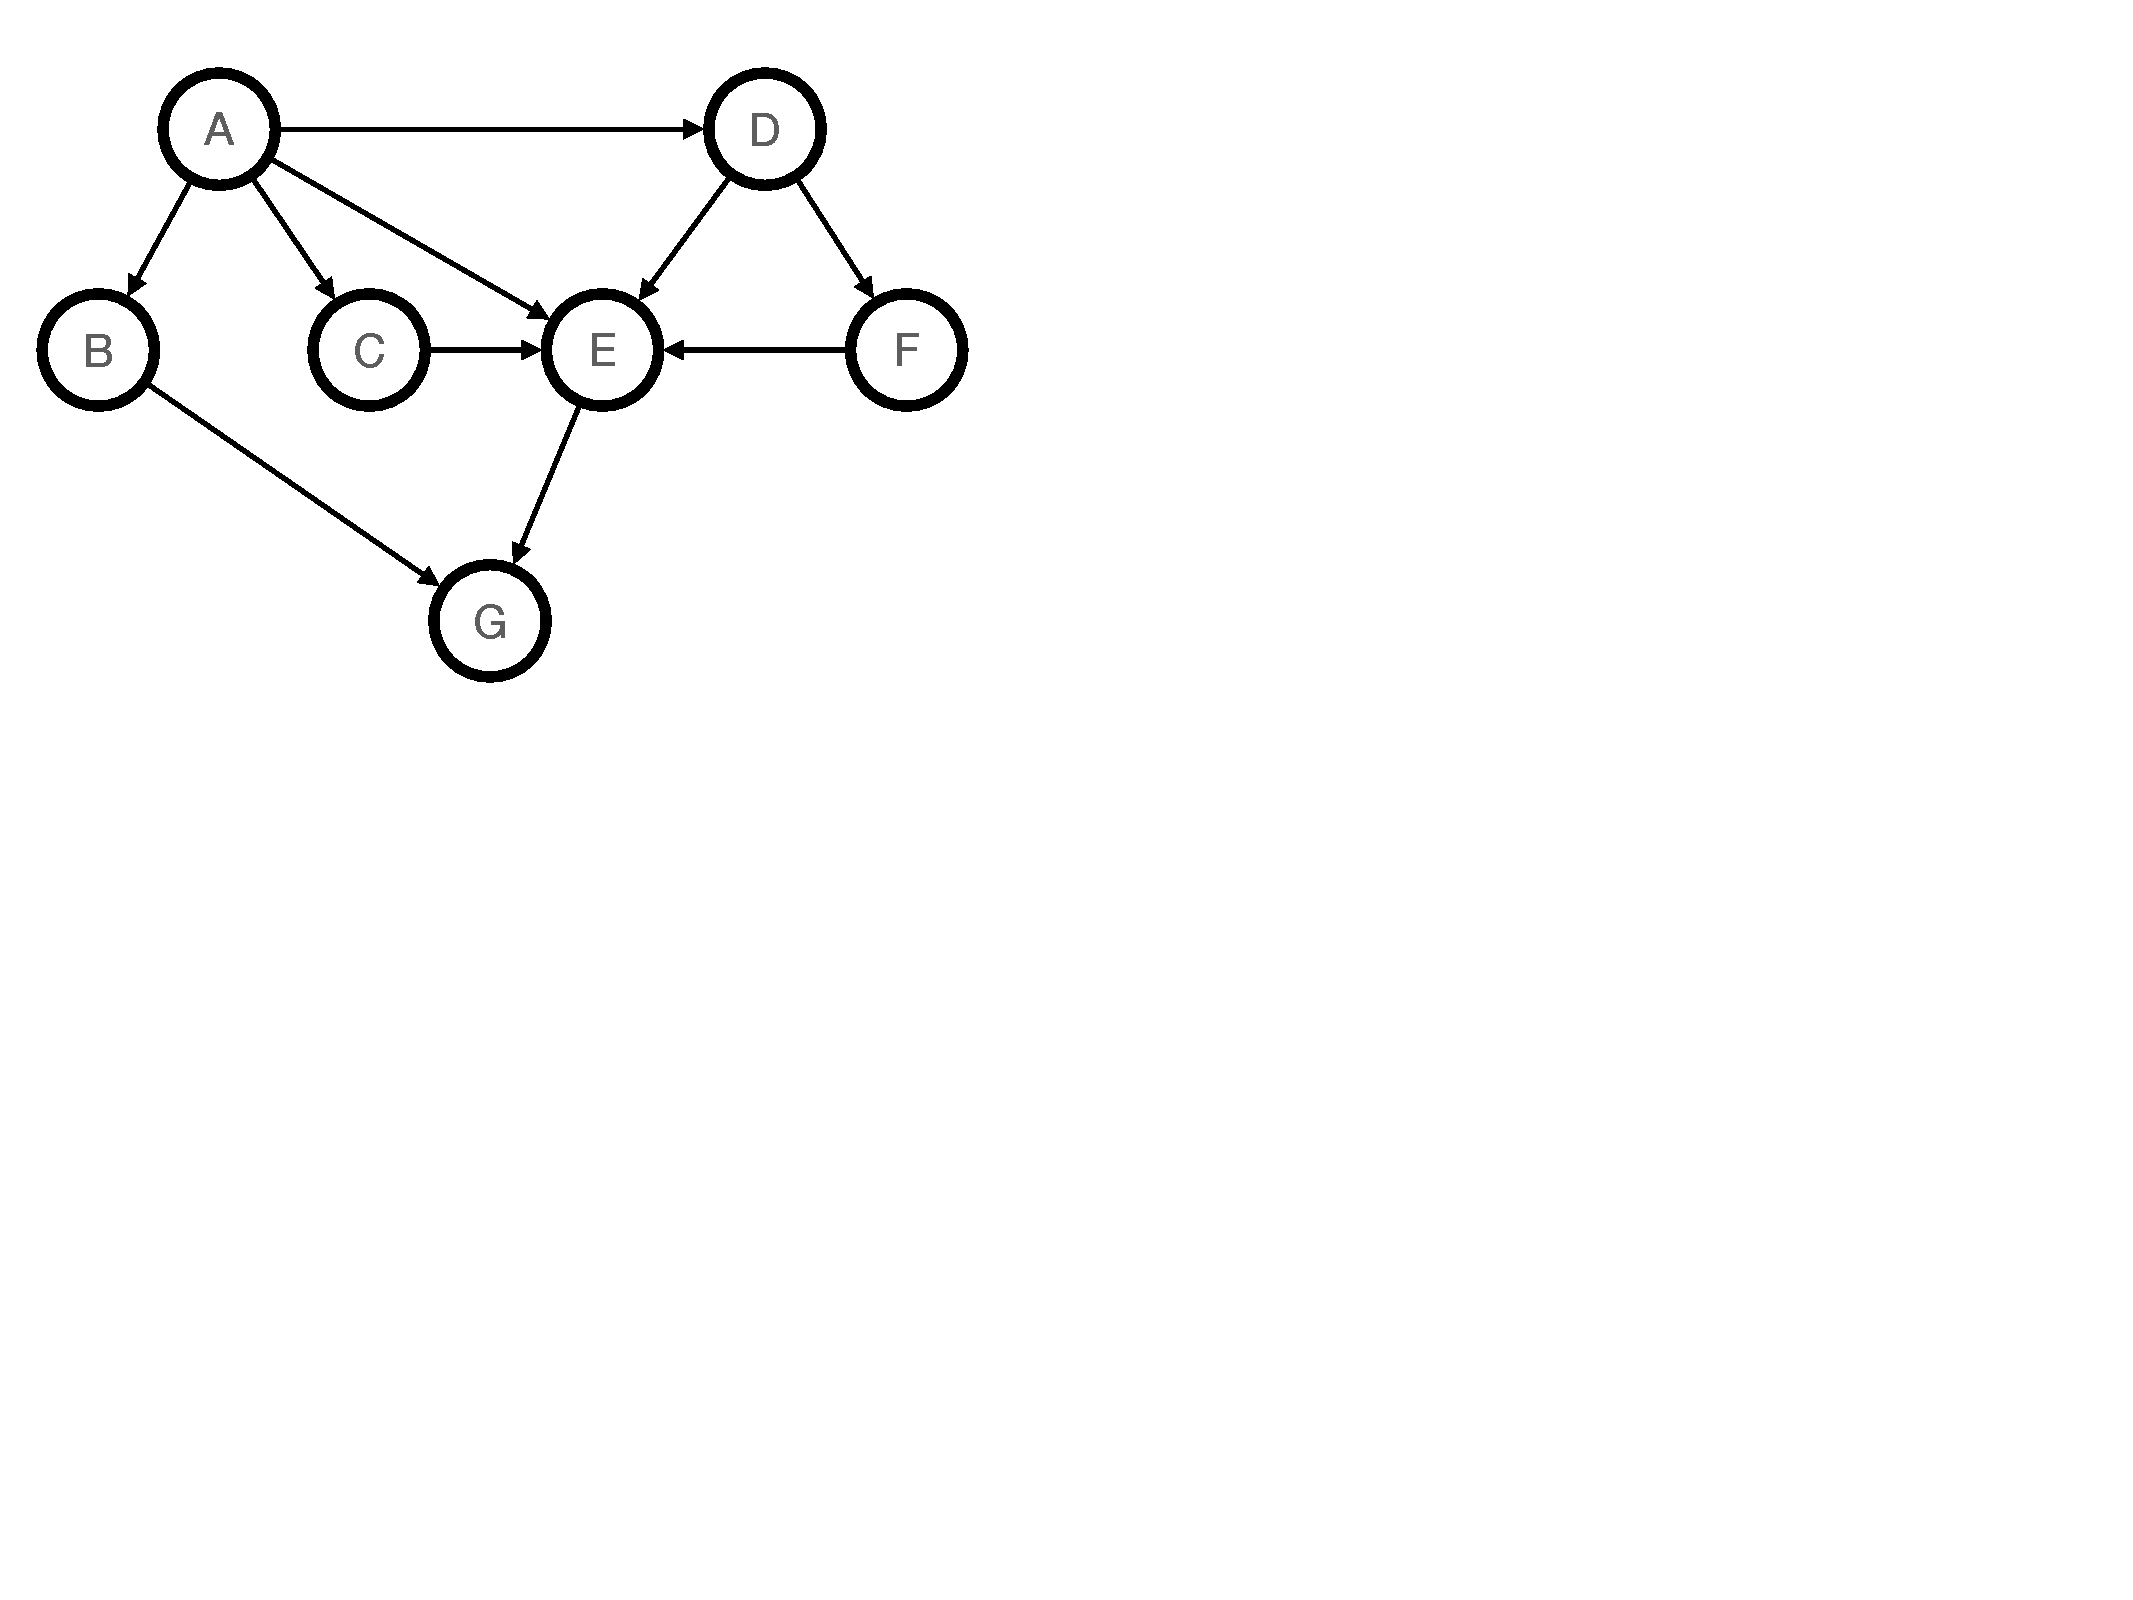
\includegraphics[width=.25\textwidth]{bn2a.pdf}
\end{center}

\begin{answer}{.5in}
    % Answer here
\end{answer}

\item \points[bn]{5} \label{q:joint}
Draw a belief network that is consistent with a joint distribution that factors as
$P(A,B,C,D,E) = P(A)P(B|A)P(C)P(D|A,C)P(E|B,C,D)$

For \textbf{5 bonus marks}, draw another, different belief network that is \emph{also} consistent with this factoring.

\begin{answer}{2in}
    % Answer here
\end{answer}

\item \points[bn]{3}
Suppose that every random variable in the joint distribution of question~(\ref{q:joint}) has a domain containing $8$ elements.  How many rows are needed to list the full joint distribution in an explicit table?

\begin{answer}{.5in}
    % Answer here
\end{answer}

\item \points[bn]{7}
Suppose that every random variable in the joint distribution of question~(\ref{q:joint}) has a domain containing $8$ elements.  How many rows in total are needed to list the conditional probability tables for your belief network representation?

\begin{answer}{.5in}
    % Answer here
\end{answer}
\end{enumerate}

\clearpage



%------------------------------------------------------------------------------------------
\item \question[ve]{Variable Elimination}
Consider the belief network below.

\begin{center}
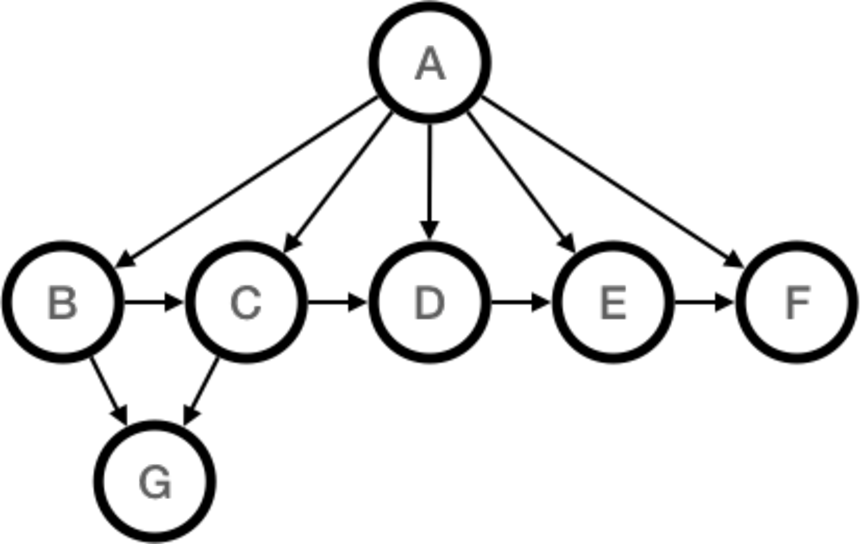
\includegraphics[width=.25\textwidth]{ve1.pdf}
\end{center}

For every variable $V$:
\begin{itemize}
\item $\operatorname{dom}(V) = \{0,1\}$
\item $\Pr(A=1) = 0.75$
\item For $V\ne A$, the probability that $V=1$ is $1-2^{-q}$, where
$q=\sum_{W\in\operatorname{parents}(V)}W$.\\
(In other words, the more of $V$'s parents have value 1, the more likely $V=1$).
\end{itemize}

\begin{enumerate}
\item\points[ve]{5}
Write a table that fully specifies the conditional probability distribution for variable $D$ in the above belief network.

\begin{answer}{1.75in}
    % Answer here
\end{answer}

\item\points[ve]{60} \label{q:code}
Implement variable elimination in Python~3 by editing the provided \texttt{ve.py} as follows:
\begin{itemize}
\item Edit the \verb|Factor| class to implement missing functionality.
\item Edit the \verb|var_elimination| function to implement variable elimination
\item Edit the function \verb|example_bn| to return a collection of factor objects that represent the belief network above.
\end{itemize}
Run the code with the command \verb|python3 ve.py| to compute the results of the
query $\Pr(B\mid G=0,E=1)$ using variable order $G,E,A,B,C,D,F$.

What is the probability $\Pr(B=1\mid G=0,E=1)$?

\begin{answer}{2\baselineskip}
    % Answer here
\end{answer}

\item\points[ve]{10}
Give an example of a variable order that would be more efficient.
Explain why your ordering is more efficient.

\begin{answer}{2in}
    % Answer here
\end{answer}
\end{enumerate}

\clearpage

\end{enumerate}


\clearpage

\section*{Submission}
The assignment you downloaded from eClass is a single ZIP archive which includes this document as a PDF {\em and} its \LaTeX{} source as well as a Python file needed for Question~\ref{q:code}.
You are to unzip the archive into an empty directory, work on the problems and then zip the directory into a new single ZIP archive for submission.

\medskip

Each assignment is to be submitted electronically via eClass by the due date.
\textbf{Your submission must be a single ZIP file containing}:
\begin{enumerate}
\item a single PDF file with your answers;
\item file(s) with your Python code.
\end{enumerate}

To generate the PDF file with your answers you can do any of the following:

\begin{itemize}
\item
insert your answers into the provided \LaTeX{} source file between \verb|\begin{answer}| and \verb|\end{answer}|. Then run the source through \LaTeX{} to produce a PDF file;

\item print out the provided PDF file and legibly write your answers in the blank spaces under each question. Make sure you write as legibly as possible for we cannot give you any points if we cannot read your hand-writing. Then scan the pages and include the scan in your ZIP submission to be uploaded on eClass;

\item use your favourite text processor and type up your answers there. Make sure you number your answers in the same way as the questions are numbered in this assignment.
\end{itemize}

\end{document}
